%& C:\Users\CBalla\AppData\Roaming\TikzEdt\TikzEdt\023~1.0\TEMP_H~1
\begin{document}
 \begin{tikzpicture}[scale=0.55,transform shape]
     \node at (0,0) {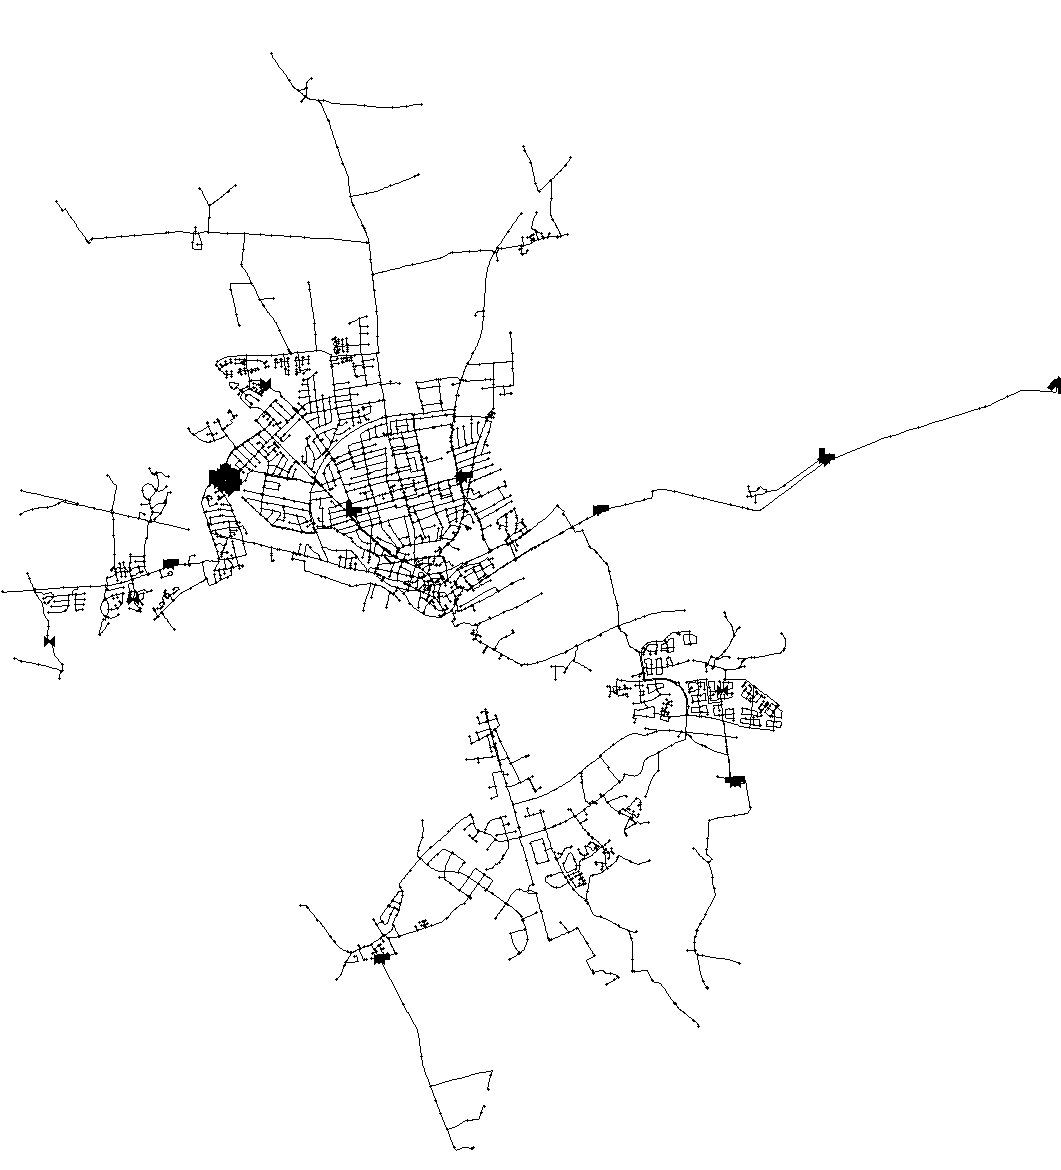
\includegraphics[width=1.5\textwidth]{verdo_pic}};

%     \node[anchor=south west,inner sep=0] at (0,0) {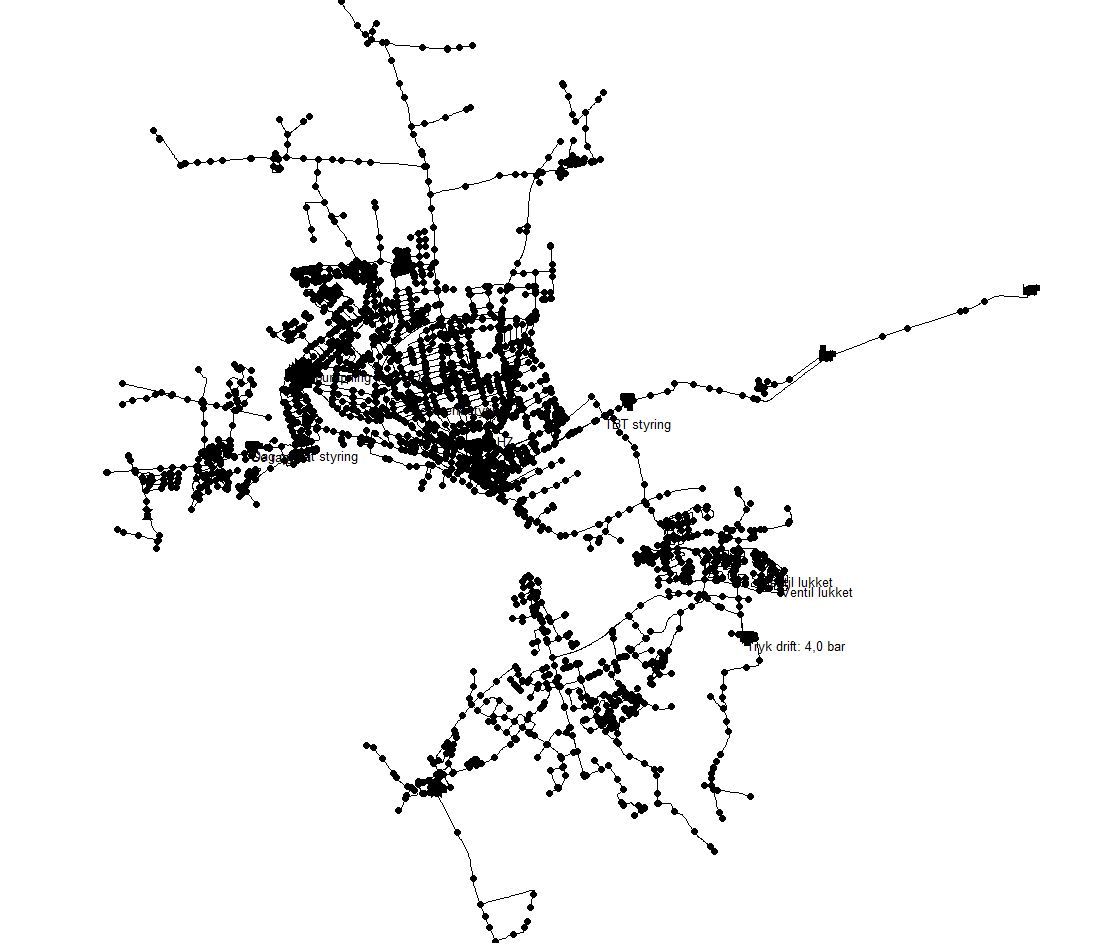
\includegraphics[width=\textwidth]{report/pictures/verdo_pic1}};
            \draw[blue,ultra thick,rounded corners] (3.55,-4.55) rectangle (4.75,-3.7);
             \draw[blue,ultra thick,rounded corners] (5.55,2.15) rectangle (6.8,3);
                      \draw[blue,ultra thick,rounded corners] (-7,2.65) rectangle (-5.75,1.8);
              \draw[blue,line width=0.65mm,rounded corners] (10.4,4.6) rectangle (11.7,3.7);
 \node[black] at (6.05,3.5) {\Large Bunkedal};
   \node[black] at (10.55,4.8) {\Large Østrup Skov};
      \node[black] at (5.6,-4.85) {\Large Vilstrup};
     \node[black] at (-8.55,3) {\Large Oust Mølle};
     
     \draw[red,ultra thick,rounded corners] (-2.1,1.85) rectangle (-0.9,2.7);
      \draw[red,ultra thick,rounded corners] (-8,-0.15) rectangle (-6.8,0.7);
           \draw[red,ultra thick,rounded corners] (1.05,1.15) rectangle (2.25,2);
                \draw[red,ultra thick,rounded corners] (-4.35,1.2) rectangle (-3.15,2.05);
                
                 \node[black] at (2.6,0.65) {\Large Toldbodgade};
                 \node[black] at (0.45,2.85) {\Large Hadsundvej};
                 \node[black] at (-6.45,-0.5) {\Large Hornbæk};
                    \node[black] at (1,5) {\Large Hobrovej};
     
 \draw [-latex](0.1,4.7) -- (-3.25,2.35);

\usetikzlibrary{calc}
\pgftransformreset
\node[inner sep=0pt,outer sep=0pt,minimum size=0pt,line width=0pt,text width=0pt,text height=0pt] at (current bounding box) {};
%add border to avoid cropping by pdflibnet
\foreach \border in {0.1}
  \useasboundingbox (current bounding box.south west)+(-\border,-\border) rectangle (current bounding box.north east)+(\border,\border);
\newwrite\metadatafile
\immediate\openout\metadatafile=\jobname_BB.txt
\path
  let
    \p1=(current bounding box.south west),
    \p2=(current bounding box.north east)
  in
  node[inner sep=0pt,outer sep=0pt,minimum size=0pt,line width=0pt,text width=0pt,text height=0pt,draw=white] at (current bounding box) {
\immediate\write\metadatafile{\p1,\p2}
};
\immediate\closeout\metadatafile
\end{tikzpicture}

\end{document}
\end{document}
t}
ing box.north east)+(\border,\border);
\newwrite\metadatafile
\immediate\openout\metadatafile=\jobname_BB.txt
\path
  let
    \p1=(current bounding box.south west),
    \p2=(current bounding box.north east)
  in
  node[inner sep=0pt,outer sep=0pt,minimum size=0pt,line width=0pt,text width=0pt,text height=0pt,draw=white] at (current bounding box) {
\immediate\write\metadatafile{\p1,\p2}
};
\immediate\closeout\metadatafile
\end{tikzpicture}

\end{document}
t}
 node[inner sep=0pt,outer sep=0pt,minimum size=0pt,line width=0pt,text width=0pt,text height=0pt,draw=white] at (current bounding box) {
\immediate\write\metadatafile{\p1,\p2}
};
\immediate\closeout\metadatafile
\end{tikzpicture}

\end{document}
ediate\closeout\metadatafile
\end{tikzpicture}

\end{document}
ediate\closeout\metadatafile
\end{tikzpicture}

\end{document}

ediate\closeout\metadatafile
\end{tikzpicture}

\end{document}

ediate\closeout\metadatafile
\end{tikzpicture}

\end{document}
t}
north east)
  in
  node[inner sep=0pt,outer sep=0pt,minimum size=0pt,line width=0pt,text width=0pt,text height=0pt,draw=white] at (current bounding box) {
\immediate\write\metadatafile{\p1,\p2}
};
\immediate\closeout\metadatafile
\end{tikzpicture}

\end{document}

pt,line width=0pt,text width=0pt,text height=0pt,draw=white] at (current bounding box) {
\immediate\write\metadatafile{\p1,\p2}
};
\immediate\closeout\metadatafile
\end{tikzpicture}

\end{document}

t}
pt,text width=0pt,text height=0pt,draw=white] at (current bounding box) {
\immediate\write\metadatafile{\p1,\p2}
};
\immediate\closeout\metadatafile
\end{tikzpicture}

\end{document}
